This question examines how the frequency of very hot days (>= 30 °C) and frost days (<= 0 °C) has changed since 1970 in three elevation‐based geographic zones:
\emph{valley} (<= 700 m), \emph{plateau} (701–1500 m), and \emph{alpine} (> 1500 m).

\subsubsection{Data Processing}
\begin{enumerate}
  \item \textbf{Load and transform:} Raw CSV data were ingested into a Spark DataFrame, with parsing of the “date” field and extraction of \texttt{year} for each station.
  \item \textbf{Parquet conversion:} The joined DataFrame (including elevation and zone labels) was repartitioned by \texttt{year} and \texttt{zone} and written to Parquet for efficient subsequent queries.
\end{enumerate}

\subsubsection{Data Analysis}
\paragraph{Full Time Series.}
We computed the annual, per‐station average counts of hot days (see Figure~\ref{fig:full_time_series_hot}) and frost days (see Figure~\ref{fig:full_time_series_frost}) for each zone.
\begin{figure}[ht]
  \centering
    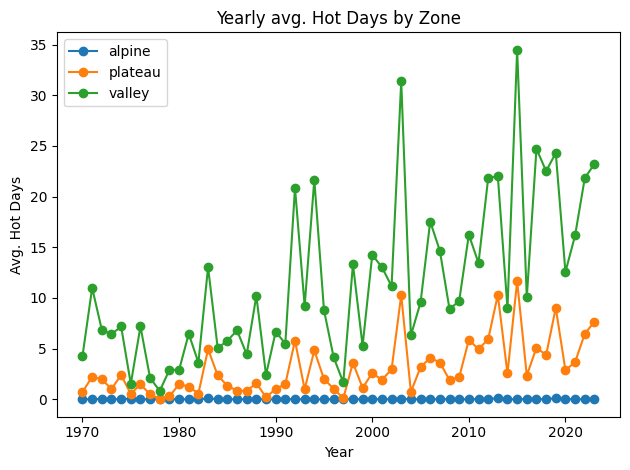
\includegraphics[width=0.45\textwidth]{img/full_time_series_hot.png}
  \caption{Yearly average hot‐day counts per station, by zone (1970–2023).}
  \label{fig:full_time_series_hot}
\end{figure}
\begin{figure}[ht]
  \centering
    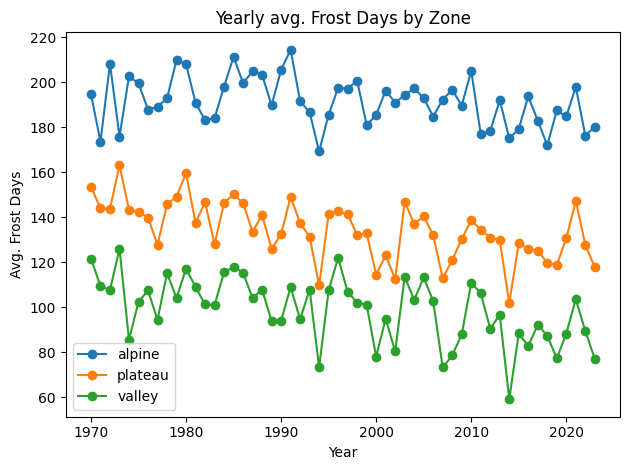
\includegraphics[width=0.45\textwidth]{img/full_time_series_frost.png}
  \caption{Yearly average frost‐day counts per station, by zone (1970–2023).}
  \label{fig:full_time_series_frost}
\end{figure}

\paragraph{End–Minus–Start Difference.}
To highlight net shifts, we compared the mean of 2014–23 vs.\ 1970–79 per zone, yielding the change in average hot‐ and frost‐days (see Figure~\ref{fig:decade_difference}).
\begin{figure}[ht]
  \centering
    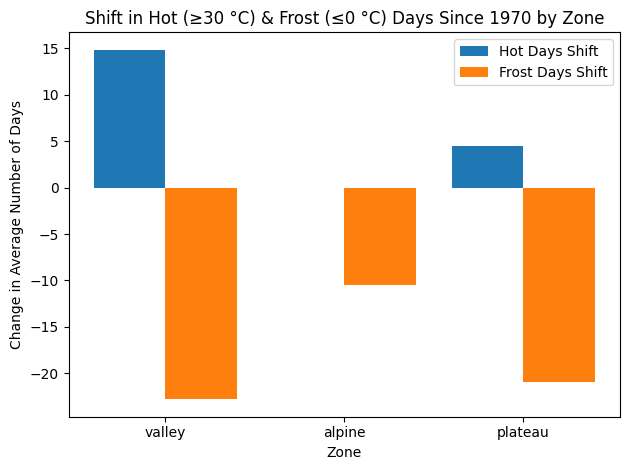
\includegraphics[width=0.45\textwidth]{img/end-minus-start_diff.png}
  \caption{Change in average hot and frost days (2014–23 minus 1970–79) by zone.}
  \label{fig:decade_difference}
\end{figure}

\paragraph{Linear Regression Trend.}
Finally, we fitted a simple linear model (OLS) of day‐count vs.\ year for each zone, extracting the slope (days per year), $R^2$, and $p$–value to quantify rate and significance of change (see Figure~\ref{fig:linear_trend}).
\begin{figure}[ht]
  \centering
    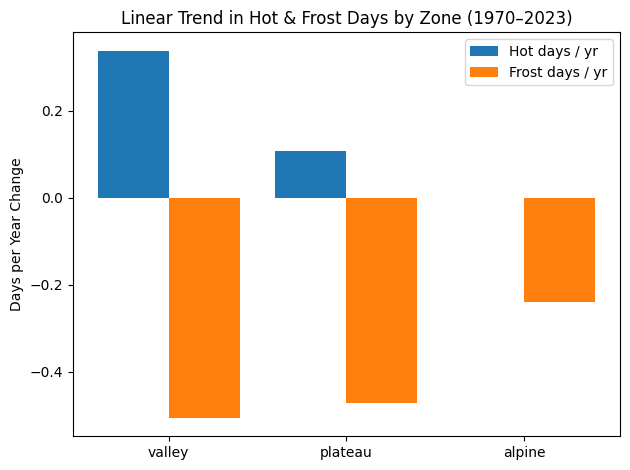
\includegraphics[width=0.45\textwidth]{img/linear_reg_trend.png}
  \caption{Estimated trend slopes in hot‐ and frost‐day counts (days per year) by zone.}
  \label{fig:linear_trend}
\end{figure}



